
\documentclass[11pt,letterpaper]{article}
\usepackage[margin=0.9in]{geometry}
\usepackage[T1]{fontenc}
\usepackage{amsmath,amssymb,graphicx,booktabs,array,url,longtable,longtable,longtable,longtable,longtable}
\usepackage[hidelinks]{hyperref}
\hypersetup{pdftitle={NeST-Com: Supplementary Configurations and Results},pdfauthor={Anonymous Authors}}
\setlength{\parindent}{0pt}\setlength{\parskip}{6pt}\emergencystretch=2em
\newcommand{\Dc}{D_c}
\begin{document}
\begin{center}\Large\bfseries NeST-Com: Fixed-Budget Next-Scale Token Communication\\[4pt]\large Supplementary Configurations and Results\end{center}
\section*{S1. Configuration and calibration}
This supplement collects the experiments and implementation records supporting the accompanying letter. The image-quality results and bootstrap intervals retain their original populations and numerical values. The current revision adds reception-conditioned summaries from existing scores, consolidates configuration evidence, and records the finite TX timing attempt in S5.1. Historical quality results, protocol checks, and their populations are preserved; no new receiver generation, training, metric evaluation, or statistical resampling is performed.

\textbf{Models and training.} NeST and WHOLE share the VAR tokenizer, VAR-d16 null-class prior, entropy coder, and adapted image decoder $\Dc$. Its adaptation uses 20\,000 ImageNet training images and continuous, fully quantized, and prefix-completion-interpolated latents. The convolutional Latent JSCC uses MSE, LPIPS, and latent-consistency losses and the same decoder; its final checkpoint is at 100k updates. SwinJSCC uses the same 20\,000 images, $256\times256$ input, paid side information, and a final 200k-update checkpoint. The selected Swin checkpoint, calibration history, training-budget stopping rule, and original training plots are available through the linked index.

\textbf{Ada adaptation.} Ada retains LlamaGen-L/VQ16 and genuine autoregressive prefix arithmetic coding. A fixed ConvNeXt predicts the class at TX; its 10-bit ID travels in the protected body, giving $b+39\leq k_a$. RX uses the recovered class and prefix. All 1--256 independently terminated prefixes are eligible. Main-curve tail generation uses CFG=4, temperature 1, top-$k=2000$, top-$p=1$, FP32 with TF32 off. The fixed single-frame adaptation does not reproduce the original long-term average-budget controller or ARQ. At N1024/19~dB all 256 tokens are sent; remaining source capacity therefore does not indicate fitting failure.

\textbf{NeST/WHOLE calibration.} The 100-image pilot uses one channel realization per source. Final evaluation uses all 1000 calibration images with three realizations per source, including fixed-gray failures. Selection maximizes DINOv2 cosine, first averaging realizations and then equally weighting sources. Exact ties use the frozen candidate order. DINO-based selection is related to feature-based evaluation; the controlled interventions separately examine the mechanism.

N1024 target screening starts at scales 7--9 and includes full-scale $(10,0)$ candidates in final evaluation. N512 screens all 7 WHOLE and 25 Quarter targets against 12 MCSs: $\log_2 M\in\{2,4,6\}$ and rates $\{1/2,2/3,3/4,5/6\}$. Each method/SNR advances the top three and a maximum-endpoint QPSK rate-1/2 anchor. Ada uses the same N512 MCS pool and up to 256 tokens. Each budget is independently calibrated; its results describe separately selected systems, rather than an isolated causal change in budget or representation order.

\href{https://github.com/daiqizai/var-comm/blob/93205a2e007ac587e28246cd399a531347a4f3f7/results/baseline_strength_20261011/Swin_1to19/selected_checkpoint.json}{Swin checkpoint and training status}; \href{https://github.com/daiqizai/var-comm/blob/93205a2e007ac587e28246cd399a531347a4f3f7/results/baseline_strength_20261011/training_figures_v1/training_calibration_curves.pdf}{training and calibration curves}; \href{https://github.com/daiqizai/var-comm/blob/93205a2e007ac587e28246cd399a531347a4f3f7/results/nestcom_n512_20261028_v1/protocol.json}{N512 frozen protocol}.

\clearpage\subsection*{S1.1. Frozen model, coder and policies}
The following configuration is verified against the actual NeST/WHOLE loader and formal receiver receipts. State SHA-256 prefixes identify the weights below; full hashes, file hashes, numerical flags and exact implementation paths are supplied in \path{results/nestcom_focused_review_20261029_v2/configuration_audit.json}.
\begin{center}\small\renewcommand{\arraystretch}{1.2}
\begin{tabular}{p{1.45in}p{4.75in}}\toprule
Component & Frozen setting\\\midrule
Prior & VAR-d16; null class; greedy completion without CFG\\
Tokenizer & 4096 entries; 32 latent channels; ten scales\\
Numerical route & FP32 model logits; TF32 off; deterministic kernels; flash/fused attention off\\
CDF & CPU float64 softmax; total $2^{24}$; minimum frequency one\\
Integer frequencies & $\lfloor p_i(2^{24}-4096)\rfloor+1$; all remaining mass goes to the largest-probability token (first index for a tie)\\
Arithmetic coder & 32-bit interval; independent termination per candidate\\

VAE state & \texttt{6830fc533a34d52c}\\
VAR state & \texttt{b82cb0855b24e1d0}\\
$D_c$ state & \texttt{bf1d64bf8ff7eeda}\\

Runtime & NeST/WHOLE receipt: Python 3.10.12, PyTorch 2.11.0+cu128, CUDA 12.8\\\bottomrule
\end{tabular}\end{center}
The entropy-decoding CDF does not use generation-stage CFG. These identities specify the numerical implementation; FP32 alone is not a guarantee of cross-hardware bitwise agreement.
\begin{center}\small\setlength{\tabcolsep}{8pt}
\begin{tabular}{rlrlrr}\toprule
$N$ & Method & SNR & Target & $\log_2 M$ & Rate\\\midrule

512 & Ada & 4 & 256 tokens & 2 & 2/3\\
512 & NeST & 4 & $(5,27)$ & 2 & 2/3\\
512 & WHOLE & 4 & $(6,0)$ & 2 & 2/3\\
512 & Ada & 10 & 256 tokens & 4 & 2/3\\
512 & NeST & 10 & $(7,0)$ & 4 & 2/3\\
512 & WHOLE & 10 & $(7,0)$ & 4 & 2/3\\
512 & Ada & 19 & 256 tokens & 6 & 5/6\\
512 & NeST & 19 & $(8,84)$ & 6 & 5/6\\
512 & WHOLE & 19 & $(8,0)$ & 6 & 5/6\\
1024 & Ada & 4 & 256 tokens & 2 & 2/3\\
1024 & NeST & 4 & $(7,25)$ & 2 & 2/3\\
1024 & WHOLE & 4 & $(7,0)$ & 2 & 2/3\\
1024 & Ada & 10 & 256 tokens & 4 & 2/3\\
1024 & NeST & 10 & $(8,126)$ & 4 & 2/3\\
1024 & WHOLE & 10 & $(9,0)$ & 4 & 2/3\\
1024 & Ada & 19 & 256 tokens & 6 & 5/6\\
1024 & NeST & 19 & $(10,0)$ & 6 & 5/6\\
1024 & WHOLE & 19 & $(10,0)$ & 6 & 5/6\\
\bottomrule\end{tabular}\end{center}
These are calibrated targets. Online fitting can select a shorter legal endpoint under the same MCS. SNR is in dB. Full candidate identifiers are retained in \texttt{frozen\_policies\_compact.csv}.

\clearpage\subsection*{S1.2. Six-system adaptations and selection}
The main comparison evaluates complete systems with different pretraining and adaptation. The tables distinguish these resources from the shared-model WHOLE/NeST comparison. No configuration is changed by this revision.
\begin{center}\small\renewcommand{\arraystretch}{1.15}
\begin{tabular}{p{0.95in}p{5.2in}}\toprule
System & Representation and adaptation\\\midrule
NeST / WHOLE & VAR-d16 and residual VQ tokenizer; shared adapted $D_c$. $D_c$: 20,000 ImageNet training images; continuous/full-quantized/prefix-completed interpolated latents; all components frozen at evaluation\\[5pt]
Latent JSCC & Frozen VAR tokenizer continuous 32 x 16 x 16 latent; convolutional channel encoder/decoder; shared $D_c$. 495,208 trainable communication parameters; width 64, 3 residual blocks; 20,000 training images; final 100,000 updates; MSE + 0.1 LPIPS + 0.01 standardized-latent MSE\\[5pt]
SwinJSCC & Author SA+RA architecture adapted to 256 x 256, initialized without pretrained communication weights. 20,000 training images; C6 / C13 alternating budgets; 200,000 total updates; RGB MSE; budget-capped stopping while calibration still improved\\[5pt]
BPG + LDPC & libbpg 0.9.8 / x265; 8-bit YCbCr 4:2:0, compression level 8. No neural training; image-adaptive downsampling to 256 / 128 / 64 / 32 and QP search 0--51\\[5pt]
ARPC adapted & Official ARPC adapted Infinity 2B/BSQ-VAE 16 weights; BLIP caption and Flan-T5-XL text conditioning. Frozen public communication weights; fixed-frame container and actual LDPC/QAM interface; no new training\\[5pt]
Ada adapted & LlamaGen-L / VQ16; fixed ConvNeXt predicts ImageNet class. Frozen pretrained representation and prior; fixed per-image frame, actual prefix arithmetic coding and paid class; no ARQ/controller reproduction\\[5pt]
\bottomrule\end{tabular}\end{center}
The Swin run stops at its training-budget cap, not a demonstrated convergence criterion. Its original training and calibration curves remain linked in S1. The decoder adaptation for NeST/WHOLE does not define a separately trained coarse-only branch.
\clearpage\subsection*{S1.2. Transmission and calibration (continued)}
\small\renewcommand{\arraystretch}{1.1}
\begin{longtable}{p{0.9in}p{2.5in}p{2.75in}}\toprule
System & Candidates and channel mapping & Selection and receiver\\\midrule\endhead
NeST / WHOLE & N512: 25 Quarter / 7 WHOLE; N1024: family-specific targets and full-scale m = 10 candidates, S1.1. Discrete LDPC/QAM; N512 12 MCSs; N1024 frozen pool and targets in S1.1 & DINOv2 cosine; cal1000, three channel outcomes/source; 100-source pilot one outcome. Profile endpoint/MCS; body 13-bit length +16-bit CRC. Null class, greedy next-scale completion; received-token overwrite and shared $D_c$\\[6pt]
Latent JSCC & No discrete token-prefix candidates. Continuous 1024 complex symbols, per-image Es = 2 normalization; no MCS & Checkpoint calibration on 1000 images, 5 training-SNR cells, 3 noises; frozen composite loss. No predicted class or text. Learned latent recovery and frozen $D_c$; no autoregressive tail\\[6pt]
SwinJSCC & No discrete token-prefix candidates. N1024: 768 continuous data symbols plus 256 charged mask/power side-information symbols; no MCS & 1000 calibration images across 2 budgets and 6 SNRs, one noise per cell; mean RGB MSE. Mask and power side information charged within N. Learned image decoder; no token completion\\[6pt]
BPG + LDPC & Coarse QP 0, 8, 16, 24, 32, 40, 48, 51 plus integer refinement at capacity crossings; select legal minimum-MSE stream. 15 MCS catalogue: QPSK/16-/64-QAM x rates 1/3, 1/2, 2/3, 3/4, 5/6; three screened per SNR & 100 calibration images, 3 noises; maximum source-mean PSNR; initial 32-source proxy screen. Complete BPG file plus protected framing; no oracle RX size or source. Actual BPG decoding and bicubic resize to 256 x 256; rejected receptions gray\\[6pt]
ARPC adapted & 7 complete-scale endpoints; one probability pass; 16-bit group trial arithmetic coding vs raw. 12 MCSs: QPSK/16-/64-QAM x rates 1/2, 2/3, 3/4, 5/6; 2 shortlisted/SNR & 100-source, 84-strategy proxy screen, then cal1000 x 3 actual noises; maximum DINOv2 cosine. Caption and token boundaries included in lossless source container. Actual prefix plus paid caption; CFG 3, temperature 0.5, top-k 900, top-p 0.97, seed 0; full scale schedule\\[6pt]
Ada adapted & All 1--256 independently terminated raster prefixes. N1024: 6 preselected MCS/SNR combinations; N512: 12 MCS pool in S1.1 & cal1000 x 3 actual noises; maximum DINOv2 cosine, then freeze. Recovered 10-bit predicted class; body overhead 39 bits including length/CRC. CFG 4, temperature 1, top-k 2000, top-p 1 sampled tail; FP32 / TF32 off\\[6pt]
\bottomrule\end{longtable}\normalsize
BPG's final 100-source PSNR calibration differs from the 1000-source DINO calibration of the generative systems. Continuous JSCC systems do not have a token-prefix/MCS search. None of these differences is treated as an isolated representation-order effect. Full settings and source SHA-256 identities are in \texttt{six\_system\_configuration.csv} and \texttt{configuration\_evidence.json} in the V3 result directory.

\clearpage\section*{S2. Statistical populations and reception accounting}
The main population is common500; Kodak has 24 sources. The endpoint, receiver, and E1/E2 controls use the existing fixed 100-source subset, not a new independent blind test. Full source IDs, preprocessing identities, and native pixel hashes join the records. Three original outcomes are averaged within a source before equal-source means and paired differences. Percentile 95\% intervals use 10\,000 source resamples; they are pointwise, not simultaneous intervals. Marginal intervals are never subtracted.

N512 methods share the registered source/repeat AWGN identities. N1024 preserves historical noise identities and is not presented as sharing noise across every method or budget. E1/E2 reuse those actual reception states; receiver counterfactuals are not new wireless frames. The 100-source bank is matched by its complete source order, not sliced from the 500-source bank. Both registered banks use seed 2026100701. Full hashes and source orders remain in the statistical identity files.

\textbf{Main matched-SNR failures.} N1024 has no rejected or failed reconstructions in 1500 trials per method/SNR; continuous Latent JSCC has no discrete CRC rejection. N512 failures below are body-CRC rejections, retained as fixed gray in all means. Header, parser, and source-decoder rejection counts are zero. No evaluated N512 source requires a NULL frame.
\begin{center}\begin{tabular}{lrrrr}\toprule
Method & 4 dB & 10 dB & 19 dB & Trials per SNR\\\midrule
NeST & 4 & 1 & 0 & 1500\\
WHOLE & 7 & 0 & 0 & 1500\\
Ada & 5 & 0 & 0 & 1500\\\bottomrule
\end{tabular}\end{center}
\textbf{Historical no-feasible-endpoint behavior.} The evaluated implementations differ. N512 sends a paid NULL profile and two zero payload bits through the complete 68+444-symbol frame, returning gray. The frozen N1024 implementation raises an execution error when no independently terminated legal stream fits; no evaluated N1024 source encountered this case. The historical implementations and results remain unchanged. The separately versioned N1024 protocol extension and its bounded checks are documented in S7.

\textbf{Granularity and receiver controls.} Mean terminated-length checks are 3.55/5.55/9.49/17.58 for Whole/Half/Quarter/Eighth. They compare already terminated streams, not extra model forwards or measured latency. Quarter is a predefined configuration, not a demonstrated optimum. The A0/B0/C0 differences are ordered interventions on the same prefixes; they are not a universal percentage decomposition. A0 still performs prior completion. At the final scale C0 and B0 coincide because no finer context is used.


\clearpage\subsection*{S2.1. Actual formal-frame energy}
The transmitted body follows packing, LDPC/RV0 rate matching, public mask XOR, and QAM modulation. The receiver reverses the mask by changing the LLR signs before LDPC decoding. The deterministic mask uses public protocol/session/frame-counter identities; it is not secret side information. Its implementation identifier is
\path{WCL_T1_public_PCG64_SHA256_protocol_session_counter_after_RV0_v1}.

The following table joins the current formal source/policy/repetition records to their original physical-event files and stored energies. It covers 22\,500 logical frames and 20\,613 distinct physical-event paths: N1024 WHOLE/PARTIAL and N512 WHOLE/NeST/Ada at 4/10/19~dB. Each row equally weights 500 sources with three repetitions each. Every method/SNR row has 1500 distinct event paths; some paths are shared between arms, explaining the smaller cross-arm total. Method-group logical and physical-unique summaries are both provided in the CSV. No older-policy energy table substitutes for these events.

Let $\rho=E_{\mathrm{frame}}/(2N)$. The table gives its mean, population standard deviation (SD, divisor 1500), minimum and maximum, together with mean $E_{\mathrm{frame}}/N$. The corresponding SD and extremes of $E_{\mathrm{frame}}/N$ are twice those of $\rho$; all values are retained in the CSV.
\begin{center}\small\setlength{\tabcolsep}{4pt}
\begin{tabular}{rlrrrrrr}\toprule
$N$ & Method & SNR & Mean $E/N$ & Mean $\rho$ & SD $\rho$ & Min $\rho$ & Max $\rho$\\\midrule

512 & Ada & 4 & 2.000000 & 1.000000 & 0.000000 & 1.000000 & 1.000000\\
512 & Ada & 10 & 2.000208 & 1.000104 & 0.022871 & 0.939062 & 1.089062\\
512 & Ada & 19 & 1.998569 & 0.999285 & 0.026561 & 0.918155 & 1.087798\\
512 & NeST & 4 & 2.000000 & 1.000000 & 0.000000 & 1.000000 & 1.000000\\
512 & NeST & 10 & 1.999427 & 0.999713 & 0.023503 & 0.920312 & 1.068750\\
512 & NeST & 19 & 2.000920 & 1.000460 & 0.025730 & 0.909970 & 1.088170\\
512 & WHOLE & 4 & 2.000000 & 1.000000 & 0.000000 & 1.000000 & 1.000000\\
512 & WHOLE & 10 & 2.002316 & 1.001158 & 0.023419 & 0.928125 & 1.081250\\
512 & WHOLE & 19 & 2.001408 & 1.000704 & 0.025361 & 0.925223 & 1.086681\\
1024 & PARTIAL & 4 & 2.000000 & 1.000000 & 0.000000 & 1.000000 & 1.000000\\
1024 & PARTIAL & 10 & 2.001052 & 1.000526 & 0.017186 & 0.945312 & 1.057031\\
1024 & PARTIAL & 19 & 2.000258 & 1.000129 & 0.018466 & 0.930617 & 1.063058\\
1024 & WHOLE & 4 & 2.000000 & 1.000000 & 0.000000 & 1.000000 & 1.000000\\
1024 & WHOLE & 10 & 2.000459 & 1.000230 & 0.017047 & 0.945312 & 1.057031\\
1024 & WHOLE & 19 & 1.999787 & 0.999894 & 0.018440 & 0.930617 & 1.063058\\
\bottomrule\end{tabular}\end{center}

All 4500 N512/4~dB logical frames use QPSK and have exactly $E_{\mathrm{frame}}=1024$ and $\rho=1$; the 68 header symbols each have energy two. Higher-order QAM exhibits finite-frame energy variation. The largest absolute paired-arm ratio of mean energies below is 0.0063~dB; the means are close without asserting equality of individual frame energies.
\clearpage
\begin{center}\small\setlength{\tabcolsep}{6pt}
\begin{tabular}{rrrrr}\toprule
$N$ & SNR & $10\log_{10}(\bar E_P/\bar E_W)$ (dB) & Mean $\Delta\rho$ & $r(\Delta E,\Delta p)$\\\midrule

512 & 4 & +0.000000 & +0.000000 & ---\\
512 & 10 & -0.006272 & -0.001445 & +0.0332\\
512 & 19 & -0.001060 & -0.000244 & +0.0335\\
1024 & 4 & +0.000000 & +0.000000 & ---\\
1024 & 10 & +0.001287 & +0.000296 & -0.0144\\
1024 & 19 & +0.001023 & +0.000235 & -0.0259\\
\bottomrule\end{tabular}\end{center}

Here $P$ is PARTIAL/NeST, $W$ is WHOLE, and $p$ is the zero-padding fraction of body information bits. The paired quantities use the same source/repetition identities; $r$ is a descriptive Pearson correlation across the 1500 pairs. A dash denotes zero energy variance. Across the nonconstant method/SNR groups, the absolute correlation between $\rho$ and padding fraction is at most 0.042. These summaries characterize the recorded transmissions; no per-frame normalization or new power-matched experiment was introduced.
\subsection*{S2.2. Actual endpoints and retained source content}
At N512/10~dB, WHOLE and NeST share target $(7,0)$ and 16-QAM rate 2/3. Direct checks of all three repetitions confirm that every source has the same TX endpoint across its repeats. The following counts are therefore source counts, not independent frame observations.
\begin{center}\begin{tabular}{rrr}\toprule
Actual endpoint & WHOLE sources & NeST sources\\\midrule

$(6,0)$ & 498 & 53\\
$(6,16)$ & 0 & 378\\
$(6,32)$ & 0 & 59\\
$(6,48)$ & 0 & 8\\
$(7,0)$ & 2 & 2\\
\midrule Total & 500 & 500\\\bottomrule\end{tabular}\end{center}

Both methods fall back from the target on 498/500 sources (99.6\%). NeST retains a within-scale endpoint on 445/500 (89.0\%). The first six scales contain 91 tokens and the seventh contains 64. Mean retained-token counts are 91.256 for WHOLE and 107.896 for NeST, a difference of 16.640. Source-bit utilization rises from 79.30\% to 93.46\%. The finer fallback retains additional information even when a full next scale does not fit; it does not reduce the target-fallback rate at this point.

The N1024 matched-SNR gain occurs with zero rejections in both families at every tested SNR. At N512/19~dB, both have zero rejections and NeST still gains 0.792~dB. At N512/10~dB, NeST has one additional body-CRC rejection yet gains 0.399~dB in the unconditional mean. These observations retain all fixed-gray failures and do not replace the primary population with a success-only subset.

Full-precision energies, paired energy differences, padding correlations, failure counts, source/endpoint counts, original-file hashes and the logical-to-physical mapping are in
\path{results/nestcom_focused_review_20261029_v2/}.

\clearpage\subsection*{S2.3. Quality decomposition by reception status}
These calculations use only the existing N512 native-array metric scores; no decoder, metric model, channel, or bootstrap is run. Every method/SNR has 500 sources and three repetitions. With frame-equal success and failure means,
\[Q_{\rm all}=p_{\rm success}Q_{\rm success}+(1-p_{\rm success})Q_{\rm failure}.\]
Because each source has three outcomes, the original equal-source overall mean equals this frame-equal mean. The maximum numerical residual of the identity over all 36 cells is $1.12\times10^{-16}$. Gray-image scores are taken from each actual failed event; they need not be equal across sources. A dash means no failed frame, with zero weighted failure term.
\textbf{LPIPS-Alex}\begin{center}\small\begin{tabular}{llrrrr}\toprule Method & SNR & Success/1500 & Overall & Success frames & Failed frames\\\midrule
ADA & 4 & 1495 & 0.554156 & 0.552943 & 0.916893\\
ADA & 10 & 1500 & 0.410977 & 0.410977 & --\\
ADA & 19 & 1500 & 0.214568 & 0.214568 & --\\
NEST & 4 & 1496 & 0.365175 & 0.363679 & 0.924583\\
NEST & 10 & 1499 & 0.272596 & 0.272076 & 1.052495\\
NEST & 19 & 1500 & 0.190053 & 0.190053 & --\\
WHOLE & 4 & 1493 & 0.395124 & 0.392485 & 0.958144\\
WHOLE & 10 & 1500 & 0.288079 & 0.288079 & --\\
WHOLE & 19 & 1500 & 0.217542 & 0.217542 & --\\
\bottomrule\end{tabular}\end{center}
\textbf{DreamSim}\begin{center}\small\begin{tabular}{llrrrr}\toprule Method & SNR & Success/1500 & Overall & Success frames & Failed frames\\\midrule
ADA & 4 & 1495 & 0.384728 & 0.382844 & 0.948163\\
ADA & 10 & 1500 & 0.258171 & 0.258171 & --\\
ADA & 19 & 1500 & 0.107753 & 0.107753 & --\\
NEST & 4 & 1496 & 0.281865 & 0.280131 & 0.930711\\
NEST & 10 & 1499 & 0.192165 & 0.191687 & 0.909004\\
NEST & 19 & 1500 & 0.121676 & 0.121676 & --\\
WHOLE & 4 & 1493 & 0.324663 & 0.321794 & 0.936442\\
WHOLE & 10 & 1500 & 0.204857 & 0.204857 & --\\
WHOLE & 19 & 1500 & 0.145797 & 0.145797 & --\\
\bottomrule\end{tabular}\end{center}
\clearpage\subsection*{S2.3. Quality decomposition (continued)}
\textbf{PSNR (dB)}\begin{center}\small\begin{tabular}{llrrrr}\toprule Method & SNR & Success/1500 & Overall & Success frames & Failed frames\\\midrule
ADA & 4 & 1495 & 11.318311 & 11.314918 & 12.332928\\
ADA & 10 & 1500 & 13.164679 & 13.164679 & --\\
ADA & 19 & 1500 & 17.690030 & 17.690030 & --\\
NEST & 4 & 1496 & 15.498715 & 15.507571 & 12.186599\\
NEST & 10 & 1499 & 17.219878 & 17.219739 & 17.428954\\
NEST & 19 & 1500 & 19.429779 & 19.429779 & --\\
WHOLE & 4 & 1493 & 15.106545 & 15.120288 & 12.175318\\
WHOLE & 10 & 1500 & 16.821305 & 16.821305 & --\\
WHOLE & 19 & 1500 & 18.637774 & 18.637774 & --\\
\bottomrule\end{tabular}\end{center}
\textbf{CLIP-I}\begin{center}\small\begin{tabular}{llrrrr}\toprule Method & SNR & Success/1500 & Overall & Success frames & Failed frames\\\midrule
ADA & 4 & 1495 & 0.789210 & 0.790088 & 0.526638\\
ADA & 10 & 1500 & 0.825748 & 0.825748 & --\\
ADA & 19 & 1500 & 0.872282 & 0.872282 & --\\
NEST & 4 & 1496 & 0.765689 & 0.766235 & 0.561732\\
NEST & 10 & 1499 & 0.814979 & 0.815175 & 0.521134\\
NEST & 19 & 1500 & 0.864000 & 0.864000 & --\\
WHOLE & 4 & 1493 & 0.746943 & 0.748068 & 0.507109\\
WHOLE & 10 & 1500 & 0.807443 & 0.807443 & --\\
WHOLE & 19 & 1500 & 0.848354 & 0.848354 & --\\
\bottomrule\end{tabular}\end{center}
\clearpage\subsection*{S2.3. Joint-success source-paired comparisons}
For each comparison, events are joined by complete source ID and original repetition identity. Only events where both methods succeed are retained. Differences are averaged over the available joint-success repetitions within each source, then equally over sources. These are descriptive conditional comparisons with no new confidence interval; they do not replace the failure-inclusive primary estimates.
\begin{center}\small\begin{tabular}{llrrrr}\toprule Comparison & SNR & Joint frames & Sources & Two repeats & Three repeats\\\midrule
NEST-WHOLE & 4 & 1493 & 500 & 7 & 493\\
NEST-WHOLE & 10 & 1499 & 500 & 1 & 499\\
NEST-WHOLE & 19 & 1500 & 500 & 0 & 500\\
NEST-ADA & 4 & 1491 & 500 & 9 & 491\\
NEST-ADA & 10 & 1499 & 500 & 1 & 499\\
NEST-ADA & 19 & 1500 & 500 & 0 & 500\\
\bottomrule\end{tabular}\end{center}
Every source retains at least two jointly successful repeats; no source is discarded.
\begin{center}\small\begin{tabular}{llrrrr}\toprule Comparison & SNR & $\Delta$LPIPS & $\Delta$DreamSim & $\Delta$PSNR & $\Delta$CLIP-I\\\midrule
NEST-WHOLE & 4 & -0.02894 & -0.04174 & +0.38886 & +0.01825\\
NEST-WHOLE & 10 & -0.01602 & -0.01315 & +0.39936 & +0.00773\\
NEST-WHOLE & 19 & -0.02749 & -0.02412 & +0.79200 & +0.01565\\
NEST-ADA & 4 & -0.18923 & -0.10249 & +4.19030 & -0.02398\\
NEST-ADA & 10 & -0.13891 & -0.06646 & +4.05598 & -0.01057\\
NEST-ADA & 19 & -0.02451 & +0.01392 & +1.73975 & -0.00828\\
\bottomrule\end{tabular}\end{center}
The LPIPS and DreamSim directions agree with the original all-event contrasts at all reported cells. Thus the observed quality differences persist on joint successes; the comparison still includes the differing models and training of each complete system. Files: \texttt{success\_failure\_quality.csv}, \texttt{joint\_success\_paired\_quality.csv}, and the source-level differences and identity JSON in the V3 \texttt{reception/} directory.

\clearpage\subsection*{S2.4. Perceptual endpoint and receiver evidence}
The following are existing source-paired bootstrap results, reorganized for the perceptual-reconstruction narrative. No statistic is recomputed. All common500 LPIPS and DreamSim intervals favor NeST/within-scale transmission at both budgets and all three SNRs. This claim does not extend to every dataset or metric; the N1024 common500 pair file does not provide CLIP-I.
\begin{center}\small\begin{tabular}{rrll}\toprule $N$ & SNR & $\Delta$LPIPS [95\% CI] & $\Delta$DreamSim [95\% CI]\\\midrule
1024 & 4 & -0.02458 [-0.02621,-0.02300] & -0.02073 [-0.02328,-0.01827]\\
1024 & 10 & -0.02725 [-0.02962,-0.02491] & -0.02405 [-0.02700,-0.02124]\\
1024 & 19 & -0.00520 [-0.00563,-0.00478] & -0.00304 [-0.00372,-0.00242]\\
512 & 4 & -0.02995 [-0.03366,-0.02640] & -0.04280 [-0.04830,-0.03734]\\
512 & 10 & -0.01548 [-0.01703,-0.01374] & -0.01269 [-0.01496,-0.01041]\\
512 & 19 & -0.02749 [-0.02883,-0.02616] & -0.02412 [-0.02639,-0.02196]\\
\bottomrule\end{tabular}\end{center}
Differences are PARTIAL/NeST minus WHOLE; populations are 500 sources, each with three original channel outcomes. The 13.7\% LPIPS and 18.3\% DreamSim reductions at N1024/10~dB describe relative changes of metric means, not percentages of human perceptual improvement.

\textbf{Controlled granularity at N1024/10~dB, 100 sources.}
\begin{center}\small\begin{tabular}{lrrrrr}\toprule Grid & Util. (\%) & LPIPS & DreamSim & PSNR & Length checks\\\midrule
Whole & 78.15 & 0.201821 & 0.131529 & 18.951576 & 3.55\\
Half & 89.21 & 0.183760 & 0.114775 & 19.395750 & 5.55\\
Quarter & 95.38 & 0.175170 & 0.107702 & 19.611725 & 9.49\\
Eighth & 97.39 & 0.172939 & 0.106972 & 19.734671 & 17.58\\
\bottomrule\end{tabular}\end{center}
Eighth--Quarter differences are LPIPS $-0.002231\,\allowbreak[-0.003228,-0.001310]$, DreamSim $-0.000730\,\allowbreak[-0.001956,0.000477]$, and PSNR $+0.122946\,\allowbreak[0.078557,0.169317]$~dB. A DreamSim interval crossing zero establishes neither equivalence nor saturation. Quarter remains the predefined main configuration.

\textbf{Ordered receiver intervention at N1024/10~dB.}
\begin{center}\small\begin{tabular}{lll}\toprule
Intervention & $\Delta$LPIPS [95\% CI] & $\Delta$DreamSim [95\% CI]\\\midrule
B0--A0 & $-0.010030\,\allowbreak[-0.012026,-0.008026]$ & $-0.008454\,\allowbreak[-0.011357,-0.005643]$\\
C0--B0 & $-0.016620\,\allowbreak[-0.020494,-0.012862]$ & $-0.015372\,\allowbreak[-0.019880,-0.011113]$\\
\bottomrule\end{tabular}\end{center}
The 100-source intervention order is fixed; these are not order-independent causal percentages. The final-scale C0--B0 effect at 19~dB is zero.

\clearpage\section*{S3. Ada tail sensitivity: $N=512$, 4 dB}
All entries use the same 100 sources and three original repetitions (300 logical results per arm). Each cell is a mean or direct paired difference with its 95\% source-bootstrap interval. Higher PSNR/CLIP-I and lower LPIPS/DreamSim are favorable.
\subsection*{Absolute metrics}
\begin{center}\small\setlength{\tabcolsep}{12pt}\renewcommand{\arraystretch}{1.55}
\begin{tabular}{lccc}
\toprule
Metric & Ada sampling & Ada argmax & NeST\\\midrule
PSNR (dB) $\uparrow$ & \shortstack{10.984\\{}[10.574, 11.410]} & \shortstack{10.509\\{}[10.099, 10.933]} & \shortstack{15.141\\{}[14.621, 15.673]}\\
LPIPS $\downarrow$ & \shortstack{0.5610\\{}[0.5457, 0.5759]} & \shortstack{0.6033\\{}[0.5857, 0.6209]} & \shortstack{0.3668\\{}[0.3511, 0.3823]}\\
DreamSim $\downarrow$ & \shortstack{0.3797\\{}[0.3523, 0.4071]} & \shortstack{0.4247\\{}[0.3966, 0.4534]} & \shortstack{0.2786\\{}[0.2591, 0.2981]}\\
CLIP-I $\uparrow$ & \shortstack{0.7922\\{}[0.7740, 0.8095]} & \shortstack{0.7661\\{}[0.7466, 0.7851]} & \shortstack{0.7658\\{}[0.7468, 0.7855]}\\
\bottomrule\end{tabular}\end{center}
\subsection*{Direct source-paired differences}
\begin{center}\small\setlength{\tabcolsep}{7pt}\renewcommand{\arraystretch}{1.55}
\begin{tabular}{lccc}
\toprule
Metric & \shortstack{Argmax minus\\sampling} & \shortstack{NeST minus\\argmax} & \shortstack{NeST minus\\sampling}\\\midrule
PSNR (dB) $\uparrow$ & \shortstack{-0.475\\{}[-0.801, -0.152]} & \shortstack{4.632\\{}[4.183, 5.093]} & \shortstack{4.157\\{}[3.772, 4.558]}\\
LPIPS $\downarrow$ & \shortstack{0.0423\\{}[0.0294, 0.0555]} & \shortstack{-0.2365\\{}[-0.2567, -0.2167]} & \shortstack{-0.1942\\{}[-0.2100, -0.1789]}\\
DreamSim $\downarrow$ & \shortstack{0.0450\\{}[0.0282, 0.0621]} & \shortstack{-0.1461\\{}[-0.1709, -0.1218]} & \shortstack{-0.1010\\{}[-0.1248, -0.0769]}\\
CLIP-I $\uparrow$ & \shortstack{-0.0261\\{}[-0.0378, -0.0143]} & \shortstack{-0.0003\\{}[-0.0194, 0.0185]} & \shortstack{-0.0263\\{}[-0.0449, -0.0078]}\\
\bottomrule\end{tabular}\end{center}
Fixed-gray counts per 300: Ada-sampling: 0, Ada-argmax: 0, NeST: 1.
The deterministic tail lowers Ada PSNR and worsens its three feature metrics relative to sampling. NeST retains higher PSNR and lower LPIPS/DreamSim than argmax; the CLIP-I difference interval crosses zero. The sampling configuration remains the main baseline.
Only unreceived-tail token selection changes. Context/KV is rebuilt from the actual received prefix and follows each new greedy token. The paid class, CFG composition, entropy-decoding conditional CDF, model, decoder, and numerical route remain fixed. No sampling-tail KV is reused. Full-token receptions reuse the existing output exactly; failed/NULL inputs remain gray.
\clearpage\section*{S3. Ada tail sensitivity: $N=512$, 10 dB}
All entries use the same 100 sources and three original repetitions (300 logical results per arm). Each cell is a mean or direct paired difference with its 95\% source-bootstrap interval. Higher PSNR/CLIP-I and lower LPIPS/DreamSim are favorable.
\subsection*{Absolute metrics}
\begin{center}\small\setlength{\tabcolsep}{12pt}\renewcommand{\arraystretch}{1.55}
\begin{tabular}{lccc}
\toprule
Metric & Ada sampling & Ada argmax & NeST\\\midrule
PSNR (dB) $\uparrow$ & \shortstack{12.878\\{}[12.384, 13.398]} & \shortstack{12.227\\{}[11.738, 12.751]} & \shortstack{16.827\\{}[16.313, 17.347]}\\
LPIPS $\downarrow$ & \shortstack{0.4121\\{}[0.3975, 0.4266]} & \shortstack{0.4416\\{}[0.4237, 0.4598]} & \shortstack{0.2818\\{}[0.2683, 0.2955]}\\
DreamSim $\downarrow$ & \shortstack{0.2511\\{}[0.2296, 0.2728]} & \shortstack{0.2856\\{}[0.2627, 0.3098]} & \shortstack{0.1955\\{}[0.1797, 0.2123]}\\
CLIP-I $\uparrow$ & \shortstack{0.8337\\{}[0.8170, 0.8502]} & \shortstack{0.8105\\{}[0.7929, 0.8278]} & \shortstack{0.8208\\{}[0.8028, 0.8386]}\\
\bottomrule\end{tabular}\end{center}
\subsection*{Direct source-paired differences}
\begin{center}\small\setlength{\tabcolsep}{7pt}\renewcommand{\arraystretch}{1.55}
\begin{tabular}{lccc}
\toprule
Metric & \shortstack{Argmax minus\\sampling} & \shortstack{NeST minus\\argmax} & \shortstack{NeST minus\\sampling}\\\midrule
PSNR (dB) $\uparrow$ & \shortstack{-0.651\\{}[-0.984, -0.338]} & \shortstack{4.600\\{}[4.188, 5.018]} & \shortstack{3.949\\{}[3.566, 4.348]}\\
LPIPS $\downarrow$ & \shortstack{0.0296\\{}[0.0201, 0.0394]} & \shortstack{-0.1598\\{}[-0.1754, -0.1439]} & \shortstack{-0.1302\\{}[-0.1429, -0.1178]}\\
DreamSim $\downarrow$ & \shortstack{0.0345\\{}[0.0232, 0.0461]} & \shortstack{-0.0901\\{}[-0.1120, -0.0689]} & \shortstack{-0.0556\\{}[-0.0760, -0.0360]}\\
CLIP-I $\uparrow$ & \shortstack{-0.0231\\{}[-0.0337, -0.0128]} & \shortstack{0.0102\\{}[-0.0072, 0.0280]} & \shortstack{-0.0129\\{}[-0.0300, 0.0039]}\\
\bottomrule\end{tabular}\end{center}
Fixed-gray counts per 300: Ada-sampling: 0, Ada-argmax: 0, NeST: 1.
The deterministic tail lowers Ada PSNR and worsens its three feature metrics relative to sampling. NeST retains higher PSNR and lower LPIPS/DreamSim than argmax; the CLIP-I difference interval crosses zero. The sampling configuration remains the main baseline.
Only unreceived-tail token selection changes. Context/KV is rebuilt from the actual received prefix and follows each new greedy token. The paid class, CFG composition, entropy-decoding conditional CDF, model, decoder, and numerical route remain fixed. No sampling-tail KV is reused. Full-token receptions reuse the existing output exactly; failed/NULL inputs remain gray.
\clearpage\section*{S3. Ada tail sensitivity: $N=1024$, 10 dB}
All entries use the same 100 sources and three original repetitions (300 logical results per arm). Each cell is a mean or direct paired difference with its 95\% source-bootstrap interval. Higher PSNR/CLIP-I and lower LPIPS/DreamSim are favorable.
\subsection*{Absolute metrics}
\begin{center}\small\setlength{\tabcolsep}{12pt}\renewcommand{\arraystretch}{1.55}
\begin{tabular}{lccc}
\toprule
Metric & Ada sampling & Ada argmax & NeST\\\midrule
PSNR (dB) $\uparrow$ & \shortstack{19.200\\{}[18.592, 19.824]} & \shortstack{19.044\\{}[18.403, 19.698]} & \shortstack{19.612\\{}[19.083, 20.146]}\\
LPIPS $\downarrow$ & \shortstack{0.1717\\{}[0.1596, 0.1845]} & \shortstack{0.1755\\{}[0.1625, 0.1890]} & \shortstack{0.1752\\{}[0.1653, 0.1851]}\\
DreamSim $\downarrow$ & \shortstack{0.0863\\{}[0.0795, 0.0933]} & \shortstack{0.0899\\{}[0.0823, 0.0978]} & \shortstack{0.1077\\{}[0.1000, 0.1157]}\\
CLIP-I $\uparrow$ & \shortstack{0.8897\\{}[0.8764, 0.9023]} & \shortstack{0.8884\\{}[0.8751, 0.9008]} & \shortstack{0.8759\\{}[0.8607, 0.8905]}\\
\bottomrule\end{tabular}\end{center}
\subsection*{Direct source-paired differences}
\begin{center}\small\setlength{\tabcolsep}{7pt}\renewcommand{\arraystretch}{1.55}
\begin{tabular}{lccc}
\toprule
Metric & \shortstack{Argmax minus\\sampling} & \shortstack{NeST minus\\argmax} & \shortstack{NeST minus\\sampling}\\\midrule
PSNR (dB) $\uparrow$ & \shortstack{-0.156\\{}[-0.369, 0.057]} & \shortstack{0.568\\{}[0.246, 0.902]} & \shortstack{0.412\\{}[0.157, 0.677]}\\
LPIPS $\downarrow$ & \shortstack{0.0038\\{}[0.0007, 0.0071]} & \shortstack{-0.0003\\{}[-0.0072, 0.0062]} & \shortstack{0.0034\\{}[-0.0021, 0.0089]}\\
DreamSim $\downarrow$ & \shortstack{0.0036\\{}[0.0010, 0.0060]} & \shortstack{0.0178\\{}[0.0129, 0.0229]} & \shortstack{0.0214\\{}[0.0167, 0.0262]}\\
CLIP-I $\uparrow$ & \shortstack{-0.0013\\{}[-0.0052, 0.0025]} & \shortstack{-0.0124\\{}[-0.0222, -0.0025]} & \shortstack{-0.0137\\{}[-0.0235, -0.0038]}\\
\bottomrule\end{tabular}\end{center}
Fixed-gray counts per 300: Ada-sampling: 0, Ada-argmax: 0, NeST: 0.
The argmax PSNR difference from sampling includes zero, while DreamSim becomes worse. NeST retains higher PSNR than argmax; Ada argmax retains better DreamSim and CLIP-I, and the LPIPS interval crosses zero. Decoding sensitivity does not remove other complete-system differences.
Only unreceived-tail token selection changes. Context/KV is rebuilt from the actual received prefix and follows each new greedy token. The paid class, CFG composition, entropy-decoding conditional CDF, model, decoder, and numerical route remain fixed. No sampling-tail KV is reused. Full-token receptions reuse the existing output exactly; failed/NULL inputs remain gray.

\clearpage\section*{S4. Completion versus direct coarse decoding}
R0 decodes $\Dc(\sum_{s=1}^{m}C_s(q_s))$ from the actual received WHOLE prefix. R1 is the existing VAR-completed reconstruction of that same prefix. Both retain the original ten-scale indexing, scale-dependent residual transforms, full latent grid, frozen adapted $\Dc$, clipping, and metric preprocessing. Unreceived scales contribute nothing to R0; codebook ID zero is not used as zero contribution. Neither arm uses unsent source tokens or a continuous source latent. This is distinct from A0/B0/C0, which intervene on received boundary-token use.

\textbf{Decoder training coverage.} The fixed decoder was adapted with an exact 50\% continuous-latent, 25\% fully quantized-latent, and 25\% interpolation mixture. The interpolation starts from $F_{b,\mathrm{TX}}$, a complete latent formed by \texttt{complete\_latent} from the first eight true source scales and generated subsequent scales, and moves toward the continuous latent. That training-cache completion uses the training source's class label, whereas the formal NeST receiver uses null-class greedy completion without CFG. The interpolation does not start from a coarse-only residual sum. The training code has no explicit coarse-only input branch. Sharing $\Dc$ therefore fixes the parameters but does not equalize adaptation to the two input distributions.

\subsection*{$N=512$, 4 dB: 100 sources, 300 results per arm}
\begin{center}\small\setlength{\tabcolsep}{7pt}\renewcommand{\arraystretch}{1.55}
\begin{tabular}{lccc}
\toprule
Metric & R0 coarse & R1 completed & R1 minus R0\\\midrule
PSNR (dB) $\uparrow$ & \shortstack{14.787\\{}[14.293, 15.296]} & \shortstack{14.813\\{}[14.261, 15.383]} & \shortstack{0.026\\{}[-0.204, 0.271]}\\
LPIPS $\downarrow$ & \shortstack{0.6612\\{}[0.6376, 0.6843]} & \shortstack{0.3960\\{}[0.3752, 0.4172]} & \shortstack{-0.2652\\{}[-0.2806, -0.2500]}\\
DreamSim $\downarrow$ & \shortstack{0.7369\\{}[0.7154, 0.7575]} & \shortstack{0.3166\\{}[0.2915, 0.3421]} & \shortstack{-0.4204\\{}[-0.4488, -0.3925]}\\
CLIP-I $\uparrow$ & \shortstack{0.5493\\{}[0.5337, 0.5649]} & \shortstack{0.7521\\{}[0.7303, 0.7737]} & \shortstack{0.2028\\{}[0.1837, 0.2218]}\\
\bottomrule\end{tabular}\end{center}
Fixed-gray count per arm: 3.
\subsection*{$N=512$, 10 dB: 100 sources, 300 results per arm}
\begin{center}\small\setlength{\tabcolsep}{7pt}\renewcommand{\arraystretch}{1.55}
\begin{tabular}{lccc}
\toprule
Metric & R0 coarse & R1 completed & R1 minus R0\\\midrule
PSNR (dB) $\uparrow$ & \shortstack{15.722\\{}[15.235, 16.209]} & \shortstack{16.493\\{}[15.993, 17.004]} & \shortstack{0.771\\{}[0.563, 0.986]}\\
LPIPS $\downarrow$ & \shortstack{0.5581\\{}[0.5388, 0.5771]} & \shortstack{0.2943\\{}[0.2817, 0.3068]} & \shortstack{-0.2638\\{}[-0.2774, -0.2504]}\\
DreamSim $\downarrow$ & \shortstack{0.6574\\{}[0.6335, 0.6804]} & \shortstack{0.2055\\{}[0.1897, 0.2216]} & \shortstack{-0.4519\\{}[-0.4790, -0.4248]}\\
CLIP-I $\uparrow$ & \shortstack{0.5748\\{}[0.5574, 0.5924]} & \shortstack{0.8150\\{}[0.7965, 0.8338]} & \shortstack{0.2403\\{}[0.2206, 0.2595]}\\
\bottomrule\end{tabular}\end{center}
Fixed-gray count per arm: 0.
Within this fixed adapted receiver, completion improves all three feature metrics at both points; PSNR improves clearly at 10~dB, while its 4~dB interval includes zero. This controlled switch does not establish superiority over a coarse-only decoder trained with comparable input coverage. No new decoder training was performed for this revision.

\clearpage\section*{S5. Additional results and processing cost}
\textbf{N2048.} On 100 sources, the existing experiment uses two paid 1024-symbol subframes. Complete representations at 19~dB give NeST $+1.806$~dB PSNR over ARPC, but worse DISTS\footnote{K. Ding, K. Ma, S. Wang, and E. P. Simoncelli, ``Image quality assessment: Unifying structure and texture similarity,'' \emph{IEEE Trans. Pattern Anal. Mach. Intell.}, vol. 44, no. 5, pp. 2567--2581, May 2022.}: $+0.0054\,[0.0024,0.0086]$. DISTS is an additional perceptual measure in this historical experiment, not a replacement for the four main metrics.

\textbf{SNR mismatch.} With both WHOLE/PARTIAL transmit policies fixed at 10~dB and RX using the true noise variance, all 300 receptions per method on 100 sources are rejected at 8~dB. All succeed at 10 and 12~dB; for each source and method the recovered prefix and reconstruction are identical at those two points. PARTIAL exceeds WHOLE by $0.660\,[0.515,0.814]$~dB PSNR. These tested points do not locate the rejection threshold or measure the steepness of the 8--10~dB transition.

\textbf{Processing cost.} The following software times are from an RTX PRO~6000 with six CPU cores, batch one, 16 development images, and three measured repetitions after warm-up. They are measured processing times, distinct from the count of length checks. Ada was not timed under this protocol.
\begin{center}\small\begin{tabular}{llrrr}\toprule
Method & SNR (dB) & TX mean (ms) & RX mean (ms) & Total mean (ms)\\\midrule

NeST & 4 & 185.50 & 358.71 & 544.21\\
NeST & 10 & 220.89 & 398.82 & 619.71\\
NeST & 19 & 302.35 & 472.27 & 774.62\\
Latent JSCC & 4 & 16.15 & 24.50 & 40.65\\
Latent JSCC & 10 & 17.97 & 24.51 & 42.48\\
Latent JSCC & 19 & 16.99 & 24.43 & 41.42\\
SwinJSCC & 4 & 24.02 & 18.59 & 42.61\\
SwinJSCC & 10 & 24.81 & 19.89 & 44.69\\
SwinJSCC & 19 & 24.90 & 18.43 & 43.32\\
BPG + LDPC & 4 & 2285.93 & 18.50 & 2304.43\\
BPG + LDPC & 10 & 2269.87 & 23.15 & 2293.01\\
BPG + LDPC & 19 & 2269.24 & 27.26 & 2296.50\\
ARPC + LDPC-QAM & 4 & 716.44 & 719.05 & 1435.49\\
ARPC + LDPC-QAM & 10 & 719.12 & 801.18 & 1520.30\\
ARPC + LDPC-QAM & 19 & 718.19 & 868.69 & 1586.89\\
\bottomrule\end{tabular}\end{center}
All underlying means, medians, and 95th percentiles remain in \texttt{inputs/timing\_summary.csv}.

The existing NeST timing logs also record actual sequential length-fit attempts. Each SNR below has 16 development sources and three measured repetitions (48 calls), with 48 warm-up calls excluded. This is the timing population, not common500. The 95th percentile uses linear interpolation at position $0.95(n-1)$.
\begin{center}\small\begin{tabular}{rrrrr}\toprule
SNR & Mean attempts & Median & 95th percentile & Range\\\midrule

4 & 4.7500 & 5.0 & 5.0 & 3--5\\
10 & 4.7500 & 5.0 & 5.0 & 3--5\\
19 & 4.3125 & 4.5 & 5.0 & 3--5\\
\bottomrule\end{tabular}\end{center}
These are observed candidate-length comparisons after the shared source traversal; their count is neither additional prior forward calls nor the size of the candidate catalogue.

\clearpage\subsection*{S5.1. Finite Quarter/Eighth timing: incomplete identity validation}
\textbf{Status: the planned 100-source, three-repeat benchmark is not complete.} The fixed experiment uses N1024, 10~dB, maximum endpoint $(10,0)$, 16-QAM rate 2/3, batch one, fixed CPU affinity/threads, and one shared PRO6000. The two grids are interleaved. Its cap is 4 qualification, 6 warmup, and 600 measured TX calls, with a two-hour absolute wall limit including load.

The four real-weight qualification calls matched the historical tokens, all candidate streams and CDF hashes, selected endpoint, and full waveform. The first 88 sources then passed both grids in the first measured repetition. At source position 88 (common500 index 114), fresh tokenizer tokens differed from the historical cache; CDF, stream, endpoint/payload, and waveform comparisons consequently failed. The run stopped immediately. The model weights, source archive, and numerical-route identities had passed their checks. These facts do not establish the root cause of the token discrepancy. No numerical tolerance was used to relabel the event as a pass, and no cached-token substitution or retry was made.

The run performed 187 tokenizer calls, 1870 prior-scale calls and 187 complete TX waveform calls: 4 qualification, 6 warmup, 176 validated measurement calls and one invalid measurement call. The latter remains in the ledger and raw timing CSV; 423 planned TX calls were never attempted. Both workers exited, and no RX, quality metric, noise, training, or bootstrap call was made.

\textbf{Partial diagnostic only: 88 sources, one repetition per grid.} The table excludes the invalid call and all warmup/qualification calls. It must not be combined with the full 100-source quality experiment to infer a Quarter/Eighth quality--cost frontier.
\begin{center}\small\setlength{\tabcolsep}{4pt}\begin{tabular}{lrrrrrr}\toprule
 & \multicolumn{3}{c}{Quarter (ms)} & \multicolumn{3}{c}{Eighth (ms)}\\
Component & Mean & Median & p95 & Mean & Median & p95\\\midrule
Tokenizer & 19.405 & 18.324 & 18.842 & 19.432 & 18.356 & 19.121\\
Prior/CDF/context & 248.160 & 244.817 & 255.861 & 245.131 & 245.236 & 250.648\\
Incremental AC & 12.280 & 12.176 & 12.822 & 12.088 & 12.093 & 12.466\\
Endpoint finalization & 1.904 & 1.914 & 2.022 & 3.561 & 3.593 & 3.809\\
AC + finalization & 14.184 & 14.073 & 14.790 & 15.649 & 15.682 & 16.190\\
Length lookup & 0.138 & 0.131 & 0.164 & 0.152 & 0.145 & 0.174\\
Packing/LDPC/QAM & 6.751 & 2.604 & 59.288 & 6.272 & 2.593 & 30.734\\
PHY + IPC & 7.201 & 3.055 & 59.791 & 6.713 & 3.022 & 31.199\\
Complete TX & 289.465 & 280.975 & 346.681 & 287.541 & 283.283 & 331.781\\
\bottomrule\end{tabular}\end{center}
Each validated call uses ten prior-scale calls and encodes 680 tokens once. Quarter/Eighth finalize 25/49 streams; mean length checks in this partial subset are 9.534/17.659. The full 100-source quality diagnostic retains its original 9.49/17.58 means. The partial source-paired complete-TX difference (Eighth minus Quarter) is $-1.924$~ms in mean and $+1.683$~ms in median; these shared-server, incomplete measurements support no speed-ranking claim.

Complete TX runs from resident uint8 RGB to the complete host waveform, including preprocessing/H2D, tokenizer, prior/CDF, incremental AC, non-mutating finalization, length lookup, packing/LDPC/QAM, and persistent CPU-worker IPC. Model loading, file I/O, and durable audit writes are outside the timed interval. CUDA is synchronized at the required boundaries; prior/CDF/context is wall-time attribution, not isolated kernel time. Raw calls, means/medians/p95, per-source differences, resource samples, and original failure/exit receipts are preserved in the V3 \texttt{timing/} directory. Earlier resource-gate and moved-checkpoint-path failures occurred before any scientific call and remain separately recorded.

\clearpage\section*{S6. Preserved qualitative cases and source records}
The main letter restores two existing N1024/10~dB development examples, Pastries and Dog, with full source IDs:
\begin{itemize}
\item Pastries: \path{n07860988/ILSVRC2012_val_00010848_n07860988}
\item Dog: \path{n02105641/ILSVRC2012_val_00018762_n02105641}
\end{itemize}
They are not newly sampled common500 test examples. NeST/ARPC retain historical noise identity 6201; Ada/Latent JSCC retain 2001, with Ada from its independent development-two-image event. No claim of identical AWGN vectors across these methods is made. Displayed LPIPS-Alex/DreamSim values correspond to each original native-array realization.

The N512 lamp full-field/ROI view is preserved below as a local illustration. The crop is $x\in[80,180)$, $y\in[0,100)$ in the original 256-pixel grid and is identical across methods. PSNR/LPIPS values are for each full image, not the crop. It uses N512, 10~dB, original repetition seed 6201; the already displayed lamp was selected editorially, not by a new preregistered or random rule.
\begin{center}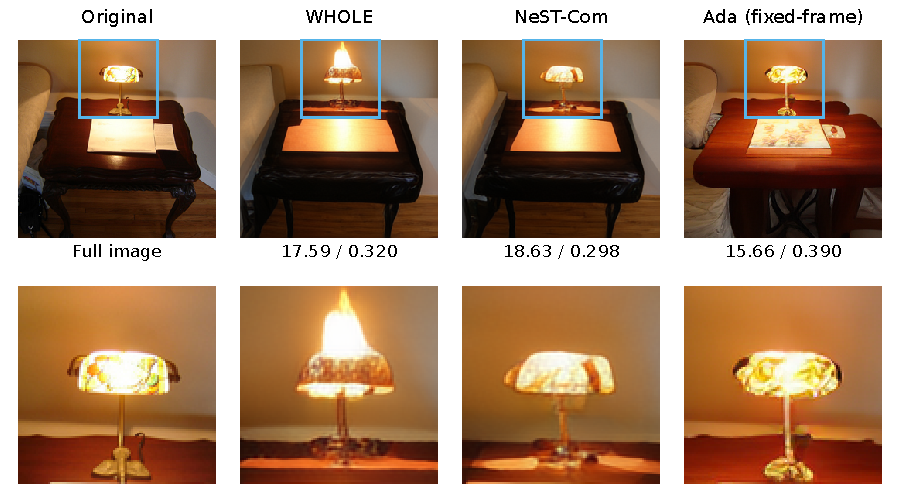
\includegraphics[width=6.0in]{supplemental/N512_lamp_roi.pdf}\end{center}
\clearpage
The earlier two-case N512 figure is also retained, with full-field images and LPIPS-Alex/DreamSim per displayed realization. Its source-ID selection history is unchanged. Both cases use N512, 10~dB, original repetition seed 6201.
\begin{center}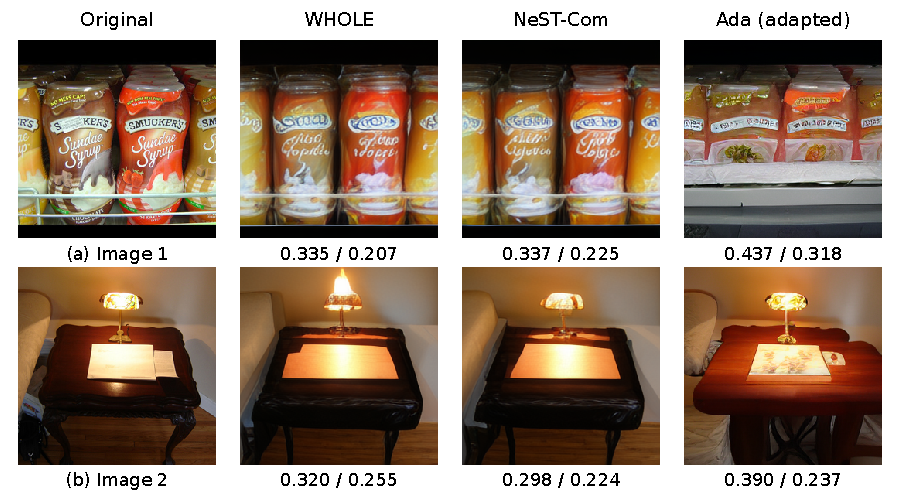
\includegraphics[width=6.0in]{supplemental/N512_previous_figure3.pdf}\end{center}
The native-array identifiers, source pixel hashes, wire inputs, display-image hashes, and full-precision metrics are retained in the source map and original selection record. No image content was enhanced or repaired.
\subsection*{Machine-readable evidence}

\href{https://github.com/daiqizai/var-comm/blob/93205a2e007ac587e28246cd399a531347a4f3f7/results/nestcom_evidence_20261029_v1/e1/REPORT_zh.md}{E1 report and complete frame/source/paired data}\par
\href{https://github.com/daiqizai/var-comm/blob/93205a2e007ac587e28246cd399a531347a4f3f7/results/nestcom_evidence_20261029_v1/e2/REPORT_zh.md}{E2 report and complete frame/source/paired data}\par
\href{https://github.com/daiqizai/var-comm/blob/93205a2e007ac587e28246cd399a531347a4f3f7/results/nestcom_evidence_20261029_v1/statistics_identity.json}{100-source statistics identity}\par
\href{https://github.com/daiqizai/var-comm/blob/93205a2e007ac587e28246cd399a531347a4f3f7/results/nestcom_n512_20261028_v1/delivery/REPORT.md}{N512 formal results and policies}\par
\href{https://github.com/daiqizai/var-comm/blob/93205a2e007ac587e28246cd399a531347a4f3f7/results/wcl_revision_20261027_v1/p1_bootstrap_clarification_v1.md}{Historical mismatch: index-only bootstrap reuse clarification}\par
\href{https://github.com/daiqizai/var-comm/blob/93205a2e007ac587e28246cd399a531347a4f3f7/results/five_method_timing_20261020_v1/delivery/summary_ms_per_image.csv}{Timing data}\par

\clearpage\section*{S7. Versioned N1024 no-fit extension}
The historical N1024 experiments used the error-on-no-fit implementation and contained no no-fit event. The independent protocol version \texttt{NESTCOM\_N1024\_PAID\_NULL\_20261029\_V2} adds paid NULL handling without changing those frozen sources or results. It preserves the original 372 profile records, header waveforms, public scrambling convention, and normal source path. Twelve appended IDs cover the original twelve MCS layouts. Missing source evidence remains an error and is not converted to NULL.

The bounded CPU checks use three historical payloads, each through the original and extended catalogues, plus twelve constructed no-fit cases covering all MCS layouts. The ordinary-path full waveforms, profiles, information/codeword hashes, and RX outputs are identical. Each no-fit case sends the full 1024-symbol frame: the paid 68-symbol header and 956-symbol body, including the 13-bit length and CRC16. The receiver recovers the explicit two-zero-bit NULL payload and returns the fixed 0.5 float gray image. Additional pure checks cover full-scale WHOLE/PARTIAL fitting and rejection guards.

Actual checks: 18 full-frame encodes, 18 full-frame receptions and 36 packet decodes; 0 source-model calls, 0 metric calls and 0 neural replays. The process exited successfully after 19.34 seconds.

Three existing image archives are hash-verified and reused because their RX inputs are identical; no new neural output equivalence is claimed from inference. These are finite noiseless-input checks with a 40~dB demapper setting. They establish targeted protocol behavior, not noisy-channel reliability or new image-quality performance. No training or resampling was performed.

The reproducible implementation and input identities are provided in:
\begin{itemize}
\item \path{experiments/nestcom-focused-review-20261029/}
\item \path{results/nestcom_focused_review_20261029_v2/nofit/}
\end{itemize}

\end{document}